\documentclass[12pt]{article}
\usepackage[a4paper, text={17cm,24cm}, top=3cm, left=1cm]{geometry}
\usepackage[utf8]{inputenc}
\usepackage{times}
\usepackage[czech]{babel}
\usepackage[unicode]{hyperref}
\usepackage{graphicx}
\usepackage{cprotect}
\usepackage{multirow}


\begin{document}

\begin{titlepage}
	\begin{center}

		
\includegraphics[height = 150pt]{img/FIT_barevne_CMYK_CZ.pdf} \\

		\begin{LARGE}
			\textsc{FAKULTA INFORMAČNÍCH TECHNOLOGIÍ} \\
			\textsc{VYSOKÉ UČENÍ TECHNICKÉ V BRNĚ}
		\end{LARGE}
		\\[5mm]
		
		\begin{LARGE}
			\textbf{Formální jazyky a překladače} 
		\end{LARGE}
        \\[20mm]
		\begin{Large}
				\textbf{Dokumentace projektu do IFJ a IAL} 
		\end{Large}
		\\[20mm]
		\begin{Large}
				\textbf{Tým 066, varianta II} 
		\end{Large}
		\\[20mm]
\begin{table}[h]
\centering
\begin{large}	
\catcode`\-=12
    \begin{tabular}{l l l l}
         Roman Ondráček & xondra58 & \% & vedoucí\\
         Pavel Raur & xraurp00 & \% &\\
         František Jeřábek & xjerab25 & \% &\\
         Radim Lipka & xlipka02 & \% & 
    \end{tabular}
\end{large}
\end{table}
\vfill
\begin{Large}
				\textbf{Seznam implementovaných rozšíření}
\end{Large}
\\[5mm]
\begin{Large}
			    \textsc{boolop, base, cycles, funexp, ifthen, tabunary} 
\end{Large}
\end{center}
\end{titlepage}

\tableofcontents
\newpage
\section{Úvod}
Tento dokument slouží jako dokumentace společného projektu do předmětů Formální jazyky a překladače a Algoritmy.
\section{Rozbor částí překladače}
\subsection{Lexikální analýza}
Lexikální analyzátor má za úkol načítat jednotlivé lexikální jednotky (lexémy) a převádět je na jednotlivé tokeny, které reprezentují daný lexém v dalších částech překladače. 

Část lexikální analýzi překledače jsme naimplementovali v modulu \textbf{scanner.c} pomocí \textit{konečného stavového automatu}, který jsme pro tuto část překladače navrhli.
Důležitou součástí lexikální analýzy překladače jazyka IFJ19 je také zásobníkový automat, který je použit pro práci s odsazením jednotlivých řádků vstupního souboru.
\begin{center}
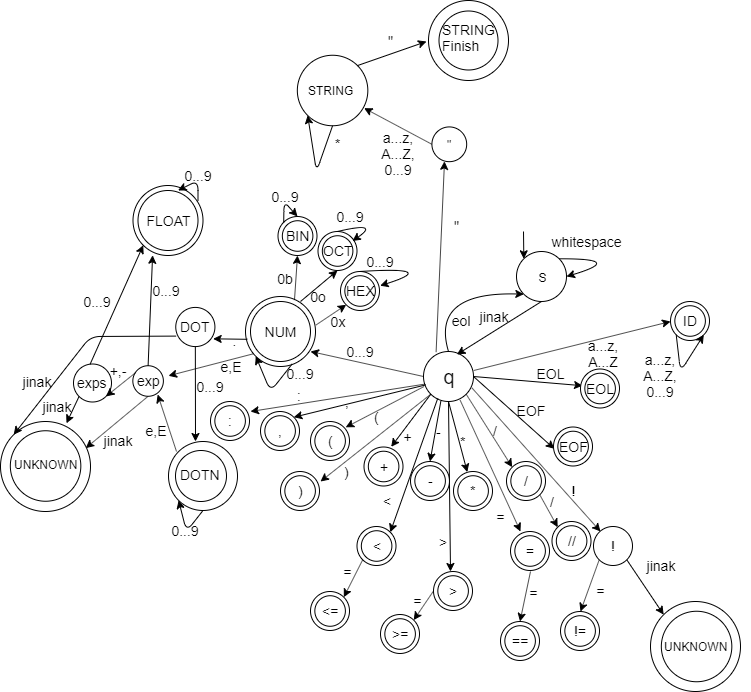
\includegraphics[height = 390pt]{img/Lexical_Analysis.png}
\end{center}
\subsection{Syntaktická analýza}
Syntaktickou analýzu jsme naimplementovali v modulu \textbf{parser.c} metodou shora dolů, konkrétněji metodou \textit{rekurzivního sestupu}, která je založena na LL--gramatice a LL--tabulce.
\subsubsection{LL--Gramatika a LL--Tabulka}
\begin{enumerate}
    \item $<$code$>$ $\rightarrow$ $<$body$>$  $<$eols$>$  $<$EOF$>$
    \item $<$body$>$ $\rightarrow$ $<$definitions$>$ $<$statements$>$
    \item $<$definitions$>$ $\rightarrow$ $<$eols$>$ $<$definition$>$ $<$definitions$>$
    \item $<$definition$>$ $\rightarrow$ $\epsilon$
    \item $<$definition$>$ $\rightarrow$ DEF IDENTIFIER ($<$function\_params$>$) : $<$eols$>$ INDENT $<$statements$>$ DEDENT
    \item $<$definition$>$ $\rightarrow$ $<$function\_call$>$
    \item $<$function\_call$>$ $\rightarrow$ IDENTIFIER ($<$function\_params$>$)
    \item $<$function\_params$>$ $\rightarrow$ $\epsilon$
    \item $<$function\_params$>$ $\rightarrow$ $<$function\_param$>$ $<$function\_nparam$>$
    \item $<$function\_nparam$>$ $\rightarrow$ , $<$function\_param$>$ $<$function\_nparam$>$
    \item $<$function\_nparam$>$ $\rightarrow$ $\epsilon$
    \item $<$function\_param$>$ $\rightarrow$ $<$expression$>$
    \item $<$statements$>$ $\rightarrow$ $\epsilon$
    \item $<$statements$>$ $\rightarrow$ $<$statement$>$ EOL $<$eols$>$ $<$statements$>$
    \item $<$statement$>$ $\rightarrow$ $<$returnRule$>$
    \item $<$statement$>$ $\rightarrow$ $<$condition$>$
    \item $<$statement$>$ $\rightarrow$ $<$asignment$>$
    \item $<$statement$>$ $\rightarrow$ $<$whileRule$>$
    \item $<$statement$>$ $\rightarrow$ PASS
    \item $<$returnRule$>$ $\rightarrow$ RETURN $<$return\_expression$>$
    \item $<$return\_expression$>$ $\rightarrow$ $\epsilon$
    \item $<$return\_expression$>$ $\rightarrow$ ($<$return\_expression$>$)
    \item $<$return\_expression$>$ $\rightarrow$ $<$expression$>$
    \item $<$condition$>$ $\rightarrow$ IF $<$condition\_expression$>$: EOL $<$eols$>$ INDENT $<$statement$>$ DEDENT $<$else\_condition$>$
    \item $<$else\_condition$>$ $\rightarrow$ $\epsilon$
    \item $<$else\_condition$>$ $\rightarrow$ ELSE : EOL $<$eols$>$ INDENT $<$statement$>$ DEDENT
    \item $<$condition\_expression$>$ $\rightarrow$ ($<$condition\_expression$>$)
    \item $<$condition\_expression$>$ $\rightarrow$ $<$expression$>$
    \item $<$asignment$>$ $\rightarrow$ IDENTIFIER = $<$expression$>$
    \item $<$whileRule$>$ $\rightarrow$ WHILE $<$condition\_expression$>$ : EOL $<$eols$>$ INDENT $<$statement$>$ DEDENT
    \item $<$eols$>$ $\rightarrow$ $\epsilon$
    \item $<$eols$>$ $\rightarrow$ EOL $<$eols$>$
\end{enumerate}
\subsubsection{Precedenční syntaktická analýza}
Precedenční syntaktická analýza je využita pro zpracování výrazů a je řízena přecedenční tabulkou. Jelikož jsme se rozhodli pro implementaci rozšíření \textsc{tabunary}, museli jsme se vypořádat s rozdílem mezi unárními operátory plus a mínus a jejich binární podobou, protože do této části syntaktické analýzy přicházejí jako od sebe nerozpoznatelné tokeny.
V precedenční analýze hojně pracujeme se zásobníkem, na který se uloží každý nově příchozí token, který následně porovnáme s vrcholem zásobníku a podle predenční tabulky provedeme náležitou operaci. Výraz se takto postupně redukuje podle redukčních pravidel a vzniká tak strom. 
\begin{table}[!htbp]
\catcode`\-=12
\centering
    \begin{tabular}{l l l}
         E $\rightarrow id$ & E $\rightarrow$ E $+$ E & E $\rightarrow$ E $<$ E \\
         E $\rightarrow $ (E) & E $\rightarrow$ E $-$ E & E $\rightarrow$ E $>$ E \\
         E $\rightarrow id$() & E $\rightarrow$ E $*$ E & E $\rightarrow$ E $<=$ E \\
         E $\rightarrow id$(E) & E $\rightarrow$ E $/$ E & E $\rightarrow$ E $>=$ E \\
         E $\rightarrow id$(E, ...) & E $\rightarrow$ E $//$ E & E $\rightarrow$ E $and$ E \\
         E $\rightarrow -$E & E $\rightarrow$ E $!=$ E & E $\rightarrow$ E $or$ E \\
         E $\rightarrow +$E & E $\rightarrow$ E $==$ E & E $\rightarrow not$ E \\
    \end{tabular}
    \caption{Redukční pravidla}
    \label{tab:1}
\end{table}
\begin{table}[!htbp]
\catcode`\-=12
\centering
    \begin{tabular}{|c|c|c|c|c|c|c|c|c|c|c|c|c|c|c|c|c|c|c|c|c|}
    \hline
       & $un+$ & $un-$ & $*$ & $/$ & $//$ & $+$ & $-$ & $<$ & $>$ & $<=$ & $>=$ & $==$ & $and$ & $or$ & $not$ & $!=$ & $($ & $)$ & $id$ & $\$$\\ 
    \hline
        $un+$ & $<$ & $<$ & $>$ & $>$ & $>$ & $>$ & $>$ & $>$ & $>$ & $>$ & $>$ & $>$ & $>$ & $>$ & $-$ & $>$ & $<$ & $>$ & $<$ & $>$\\
    \hline
        $un-$ & $<$ & $<$ & $>$ & $>$ & $>$ & $>$ & $>$ & $>$ & $>$ & $>$ & $>$ & $>$ & $>$ & $>$ & $-$ & $>$ & $<$ & $>$ & $<$ & $>$\\
    \hline
        $*$ & $<$ & $<$ & $>$ & $>$ & $>$ & $>$ & $>$ & $>$ & $>$ & $>$ & $>$ & $>$ & $>$ & $>$ & $<$ & $>$ & $<$ & $>$ & $<$ & $>$\\
    \hline
        $/$ & $<$ & $<$ & $>$ & $>$ & $>$ & $>$ & $>$ & $>$ & $>$ & $>$ & $>$ & $>$ & $>$ & $>$ & $<$ & $>$ & $<$ & $>$ & $<$ & $>$\\
    \hline
        $//$ & $<$ & $<$ & $>$ & $>$ & $>$ & $>$ & $>$ & $>$ & $>$ & $>$ & $>$ & $>$ & $>$ & $>$ & $<$ & $>$ & $<$ & $>$ & $<$ & $>$\\
    \hline
        $+$ & $<$ & $<$ & $<$ & $<$ & $<$ & $>$ & $>$ & $>$ & $>$ & $>$ & $>$ & $>$ & $>$ & $>$ & $<$ & $>$ & $<$ & $>$ & $<$ & $>$\\
    \hline
        $-$ & $<$ & $<$ & $<$ & $<$ & $<$ & $>$ & $>$ & $>$ & $>$ & $>$ & $>$ & $>$ & $>$ & $>$ & $<$ & $>$ & $<$ & $>$ & $<$ & $>$\\
    \hline
        $<$ & $<$ & $<$ & $<$ & $<$ & $<$ & $<$ & $<$ & $-$ & $-$ & $-$ & $-$ & $-$ & $>$ & $>$ & $<$ & $-$ & $<$ & $>$ & $<$ & $>$\\
    \hline
        $>$ & $<$ & $<$ & $<$ & $<$ & $<$ & $<$ & $<$ & $-$ & $-$ & $-$ & $-$ & $-$ & $>$ & $>$ & $<$ & $-$ & $<$ & $>$ & $<$ & $>$\\
    \hline
        $<=$ & $<$ & $<$ & $<$ & $<$ & $<$ & $<$ & $<$ & $-$ & $-$ & $-$ & $-$ & $-$ & $>$ & $>$ & $<$ & $-$ & $<$ & $>$ & $<$ & $>$\\
    \hline
        $>=$ & $<$ & $<$ & $<$ & $<$ & $<$ & $<$ & $<$ & $-$ & $-$ & $-$ & $-$ & $-$ & $>$ & $>$ & $<$ & $-$ & $<$ & $>$ & $<$ & $>$\\
    \hline
        $==$ & $<$ & $<$ & $<$ & $<$ & $<$ & $<$ & $<$ & $-$ & $-$ & $-$ & $-$ & $-$ & $>$ & $>$ & $<$ & $-$ & $<$ & $>$ & $<$ & $>$\\
    \hline
        $and$ & $<$ & $<$ & $<$ & $<$ & $<$ & $<$ & $<$ & $<$ & $<$ & $<$ & $<$ & $<$ & $>$ & $>$ & $<$ & $<$ & $<$ & $>$ & $<$ & $>$\\
    \hline
        $or$ & $<$ & $<$ & $<$ & $<$ & $<$ & $<$ & $<$ & $<$ & $<$ & $<$ & $<$ & $<$ & $<$ & $>$ & $<$ & $<$ & $<$ & $>$ & $<$ & $>$\\
    \hline
        $not$ & $-$ & $-$ & $>$ & $>$ & $>$ & $>$ & $>$ & $>$ & $>$ & $>$ & $>$ & $>$ & $>$ & $>$ & $<$ & $>$ & $<$ & $>$ & $<$ & $>$\\
    \hline
        $!=$ & $<$ & $<$ & $<$ & $<$ & $<$ & $<$ & $<$ & $-$ & $-$ & $-$ & $-$ & $-$ & $>$ & $>$ & $<$ & $-$ & $<$ & $>$ & $<$ & $>$\\
    \hline
        $($ & $<$ & $<$ & $<$ & $<$ & $<$ & $<$ & $<$ & $<$ & $<$ & $<$ & $<$ & $<$ & $<$ & $<$ & $<$ & $<$ & $<$ & $=$ & $<$ & $-$\\
    \hline
        $)$ & $>$ & $>$ & $>$ & $>$ & $>$ & $>$ & $>$ & $>$ & $>$ & $>$ & $>$ & $>$ & $>$ & $>$ & $>$ & $>$ & $-$ & $>$ & $-$ & $>$\\
    \hline
        $id$ & $-$ & $-$ & $>$ & $>$ & $>$ & $>$ & $>$ & $>$ & $>$ & $>$ & $>$ & $>$ & $>$ & $>$ & $>$ & $>$ & $=$ & $>$ & $-$ & $>$\\
    \hline
        $\$$ & $<$ & $<$ & $<$ & $<$ & $<$ & $<$ & $<$ & $<$ & $<$ & $<$ & $<$ & $<$ & $<$ & $<$ & $<$ & $<$ & $<$ & $-$ & $<$ & $-$\\
    \hline
    \end{tabular}
    \caption{Tabulka precedenční syntaktické analýzy}
    \label{tab:2}
\end{table}

\subsection{Sémantická analýza}
\subsection{Generátor cílového kódu}
\subsection{Optimalizace}
\section{Implementovaná rozšíření}
\subsection{BOOLOP}
\subsection{BASE}
\subsection{CYCLES}
\subsection{FUNEXP}
\subsection{IFTHEN}
\subsection{TABUNARY}
\section{Závěr}
\end{document}